% ============================================================
%  presentation.tex  —  Beamer 20-min talk
%  Stochastic Bellhop UQ — Technion SIPL
% ============================================================
\documentclass[10pt]{beamer}

\usetheme{Madrid}
\usecolortheme[RGB={0,59,126}]{structure}   % Technion blue #003B7E

\setbeamertemplate{navigation symbols}{}
\setbeamertemplate{footline}[frame number]
\setbeamertemplate{caption}[numbered]

\usepackage{amsmath,amssymb}
\usepackage{graphicx}
\usepackage{booktabs}
\usepackage{multirow}
\usepackage{subcaption}
\usepackage{xcolor}

\graphicspath{
  {../Methods/MC/}
  {../Methods/Delta/}
  {../Methods/LN3/}
  {../Methods/PCE/}
  {../Methods/Comparison/}
  {../Methods/Methods/MC/}
  {../Methods/Methods/Delta/}
  {../Methods/Methods/LN3/}
  {../Methods/Methods/PCE/}
  {../Methods/Methods/Comparison/}
  {../validation/analytical/figures/}
}

\newcommand{\EX}{\mathbb{E}}
\newcommand{\Var}{\mathrm{Var}}
\newcommand{\TL}{\mathrm{TL}}

\definecolor{technionblue}{RGB}{0,59,126}
\definecolor{successgreen}{RGB}{0,120,50}
\definecolor{failred}{RGB}{180,30,30}
\definecolor{warnyellow}{RGB}{180,120,0}

% ============================================================
\begin{document}
% ============================================================

% ── Slide 01: Title ──────────────────────────────────────────
\begin{frame}
  \titlepage
\end{frame}

\title[Stochastic TL Maps]{Uncertainty Quantification for Underwater Acoustic
       Transmission Loss}
\subtitle{Delta, PCE, LN3, and Monte Carlo Across Five Propagation Scenarios}
\author{O.~Dig}
\institute[Technion SIPL]{Signal and Image Processing Laboratory\\
          Technion --- Israel Institute of Technology}
\date{2026}

\begin{frame}
  \titlepage
\end{frame}

% ── Slide 02: Motivation ─────────────────────────────────────
\begin{frame}{Motivation: Why Probabilistic TL Prediction?}
  \begin{columns}
    \column{0.52\textwidth}
    \begin{itemize}
      \item Sonar mission planning requires \textbf{TL maps} computed by ray-tracers (Bellhop)
      \item Environmental inputs are \textbf{uncertain}: frequency tolerance, source deployment depth $z_S$, seasonal SVP variation
      \item Deterministic TL gives \emph{one} map --- \textbf{no confidence bounds}
      \item Operational failure when environment deviates from nominal
    \end{itemize}
    \vspace{0.3em}
    \begin{block}{Goal}
      Replace single-value TL with a \textbf{distribution} of TL values and compute
      $P_\mathrm{fail} = P(\TL > \mathrm{FOM})$ across the range--depth plane.
    \end{block}

    \column{0.44\textwidth}
    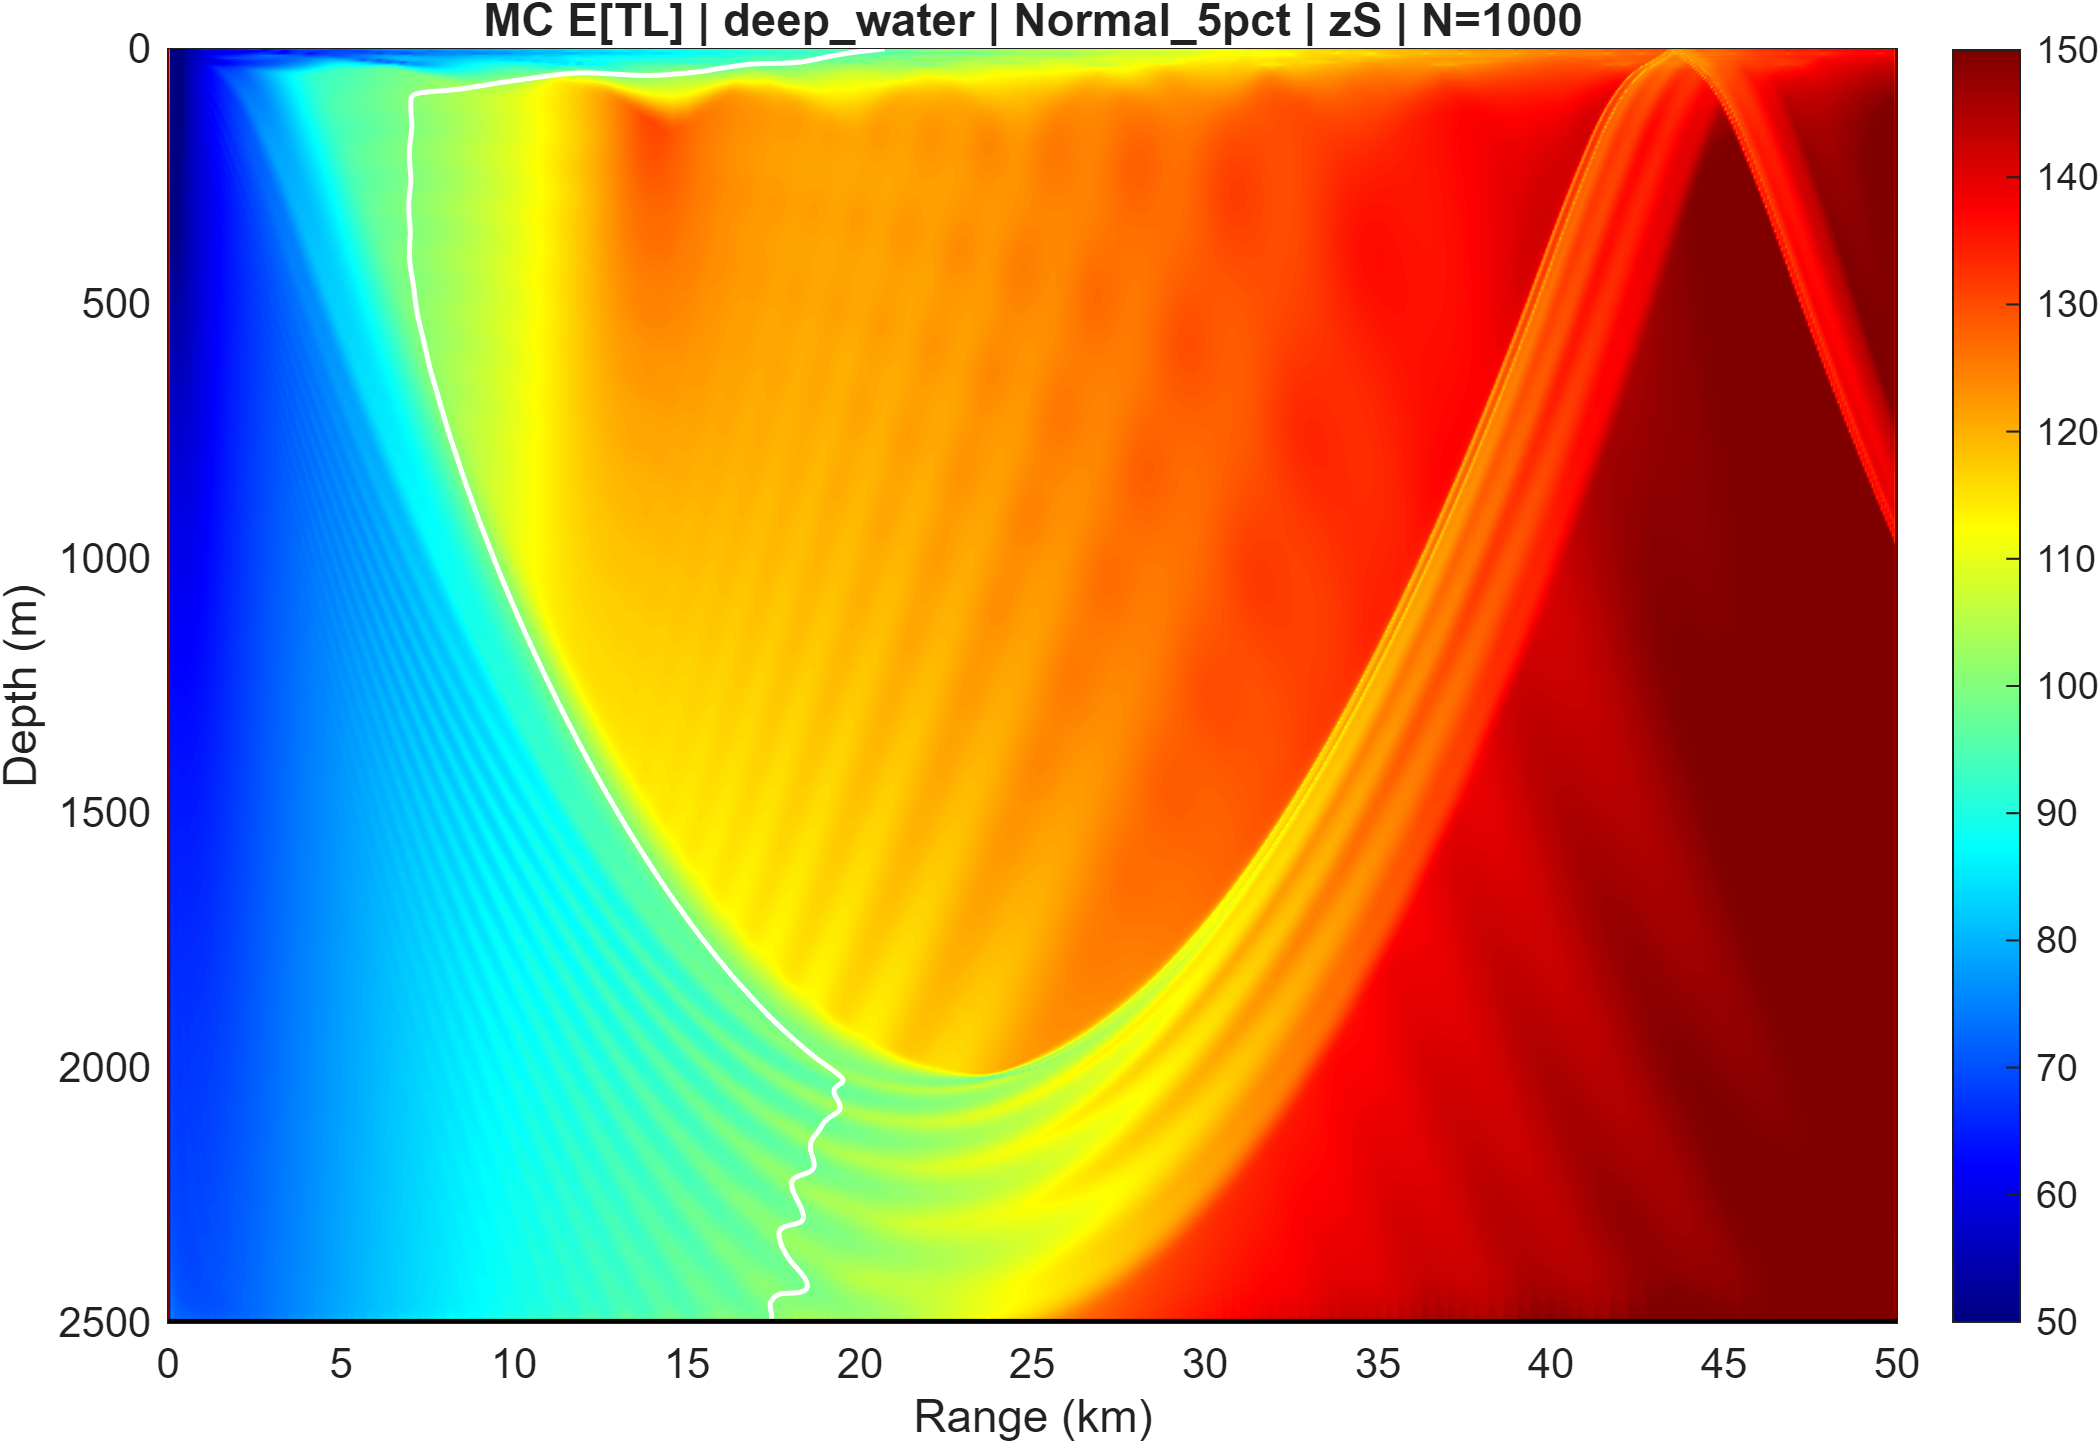
\includegraphics[width=\linewidth]{deep_water/Normal_5pct/figures/TL_zS.png}
    \captionof{figure}{\footnotesize MC mean TL, deep water, Normal\,5\% $z_S$}
  \end{columns}
\end{frame}

% ── Slide 03: The UQ Problem ─────────────────────────────────
\begin{frame}{The UQ Problem Statement}
  \begin{columns}
    \column{0.5\textwidth}
    \textbf{Uncertain inputs (3 parameters):}
    \begin{align*}
      f &\sim \mathcal{N}(\mu_f,\,\sigma_f^2),\quad \sigma_f = \tfrac{p}{200}\mu_f \\
      z_S &\sim \mathcal{N}(\mu_z,\,\sigma_z^2),\quad \sigma_z = \tfrac{p}{200}\mu_z \\
      \Delta T &\sim \mathcal{N}(0,\,\sigma_s^2)
    \end{align*}
    Uncertainty level $p \in \{1\%,\, 5\%,\, 10\%\}$

    \vspace{0.5em}
    \textbf{Five propagation scenarios:}
    \begin{itemize}\small
      \item Baseline (flat, 50\,m)
      \item Shallow water (flat, 50\,m)
      \item Deep water (flat, 2500\,m)
      \item Upslope (50\,$\to$\,20\,m)
      \item Downslope (50\,$\to$\,550\,m)
    \end{itemize}

    \column{0.46\textwidth}
    \begin{block}{Scale of the experiment}
      \begin{itemize}\small
        \item $5\text{ scenarios} \times 3\text{ distributions} \times N{=}1000$ Bellhop runs = \textbf{15,000 acoustic simulations}
        \item Grid: $N_r \times N_z = 766 \times 574 \approx 440{,}000$ pixels per run
        \item Figures: 830 PNG outputs covering all methods and scenarios
      \end{itemize}
    \end{block}
  \end{columns}
\end{frame}

% ── Slide 04: Development Journey ────────────────────────────
\begin{frame}{Development Journey: Three Phases}
  \begin{block}{Phase 1 — Archive / Exploration (Uniform distributions, baseline)}
    Small runs ($N{=}50$--100) with Uniform uncertainty to explore method sensitivity.
    Identified Delta as promising for flat geometry; motivated PCE investigation.
  \end{block}
  \vspace{0.3em}
  \begin{block}{Phase 2 — Analytical Validation}
    Validated the Bellhop Finite-Difference Jacobian (Bellhop-FD) against the
    closed-form waveguide solution.
    Established ground truth: $L_1 < 5\%$ error confirms Bellhop-FD is accurate.
  \end{block}
  \vspace{0.3em}
  \begin{block}{Phase 3 — Production Run ($N=1000$, Normal distributions)}
    Full pipeline across all 5 scenarios $\times$ 3 distributions.
    LHS+IID+SVP sampling; importance sampling for efficiency.
    Four UQ methods applied and compared to MC ground truth.
  \end{block}
\end{frame}

% ── Slide 05: Method 1 — Delta/FOSM ─────────────────────────
\begin{frame}{Method 1: Bellhop-FD Delta (FOSM / GUM Linearisation)}
  \textbf{1st-order Taylor expansion:}
  \begin{equation}
    \Var_1[\TL] \approx \sum_i J_i^2 \sigma_i^2, \quad
    J_i = \frac{\partial \TL}{\partial \theta_i}\bigg|_{\boldsymbol\theta_0}
  \end{equation}
  \begin{itemize}
    \item Jacobian $J_i$ via \textbf{Bellhop Finite-Difference}: 2 extra Bellhop runs per parameter
    \item Same method as \textbf{FOSM} (structural reliability), \textbf{GUM linearisation} (metrology)
  \end{itemize}

  \vspace{0.4em}
  \textbf{2nd-order extension:}
  \begin{equation}
    \Var_2[\TL] \approx \Var_1[\TL] + \tfrac{1}{2}\sum_i H_{ii}^2 \kappa_i \sigma_i^4
  \end{equation}

  \begin{block}{Convergence diagnostic}
    If $|\kappa H_{ii}^2|/V_1 \gg 1$, Taylor series has not converged.
    This ratio is the key indicator of Delta failure.
  \end{block}
\end{frame}

% ── Slide 06: Method 2 — PCE ─────────────────────────────────
\begin{frame}{Method 2: Polynomial Chaos Expansion (PCE)}
  \begin{columns}
    \column{0.55\textwidth}
    \textbf{Surrogate model at each pixel:}
    \begin{equation}
      \TL(\theta) \approx \sum_{n=0}^K c_n \Phi_n(\xi), \quad
      \xi = \frac{\theta - \theta_0}{\sigma}
    \end{equation}
    \begin{itemize}\small
      \item Hermite/Legendre basis $\Phi_n$ (orthogonal to input PDF)
      \item Coefficients via QR least-squares on $N{=}50$ cached MC samples
      \item \textbf{Zero new Bellhop runs required}
    \end{itemize}

    \column{0.42\textwidth}
    \textbf{Automatic order selection:}\\[3pt]
    Analytic LOO-CV without refitting:
    \begin{equation}
      e_i^\mathrm{LOO} = \frac{r_i}{1 - h_{ii}}
    \end{equation}
    \begin{equation}
      K^* = \arg\min_K\;\overline{\mathrm{LOO}}(K)
    \end{equation}
    $h_{ii}$ from QR decomposition of $\boldsymbol\Phi$ --- reused for variance too.
  \end{columns}
\end{frame}

% ── Slide 07: Method 3 — LN3 ─────────────────────────────────
\begin{frame}{Method 3: LN3 Distribution Fit}
  \textbf{Physical motivation} (CLT on mode sums):
  \begin{equation}
    p(r,z) = \sum_{m=1}^M A_m(r)\,\psi_m(z_S)\psi_m(z)
    \;\xrightarrow{M \to \infty}\; |p| \sim \text{Rayleigh}
  \end{equation}
  Converting to dB: $\TL \approx \mathrm{LN3}(\gamma, \mu, \sigma)$

  \vspace{0.4em}
  \begin{columns}
    \column{0.5\textwidth}
    \textbf{Shift parameter:}
    \begin{equation}
      \gamma = 0.95\min(\mathrm{samples})
    \end{equation}
    Encodes physical TL lower bound (geometric spreading).

    \column{0.46\textwidth}
    \textbf{Delta--LN3 hybrid:}\\
    Moments $(\mu, \sigma)$ from analytically computed
    $\EX[\TL]$ and $\Var[\TL]$.
    Shadow probability without MC:
    \begin{equation}
      P(\TL > \mathrm{FOM}) = 1 - F_\mathrm{LN3}(\mathrm{FOM})
    \end{equation}
  \end{columns}

  \vspace{0.4em}
  \begin{alertblock}{Fitting constraint}
    LHS samples are NOT i.i.d.\ --- MLE is misspecified.
    Method of moments is used (suboptimal but consistent).
  \end{alertblock}
\end{frame}

% ── Slide 08: Method 4 — MC ──────────────────────────────────
\begin{frame}{Method 4: Monte Carlo Ground Truth}
  \begin{columns}
    \column{0.52\textwidth}
    \textbf{Sampling design:}
    \begin{itemize}
      \item $N_1{=}50$ LHS + $N_2{=}50$ IID + $N_3{=}50$ SVP-perturbed = 150 per distribution
      \item Combined total: $N{=}1000$ per scenario/distribution pair
      \item Importance sampling (IS) reweights Normal\,10\% ensemble for 5\% and 1\%
    \end{itemize}

    \vspace{0.5em}
    \textbf{Convergence:}\\
    $N{=}300$ sufficient for $<5\%$ relative RMSE of $\Var[\TL]$ estimator at Normal\,10\%.

    \column{0.44\textwidth}
    
\includegraphics[width=\linewidth]{deep_water/Normal_5pct/figures/svp_ensemble.png}
    \captionof{figure}{\footnotesize SVP ensemble, deep water, Normal\,5\%, $N=1000$}
  \end{columns}
\end{frame}

% ── Slide 09: Pipeline Architecture ──────────────────────────
\begin{frame}{Pipeline Architecture}
  \begin{center}
    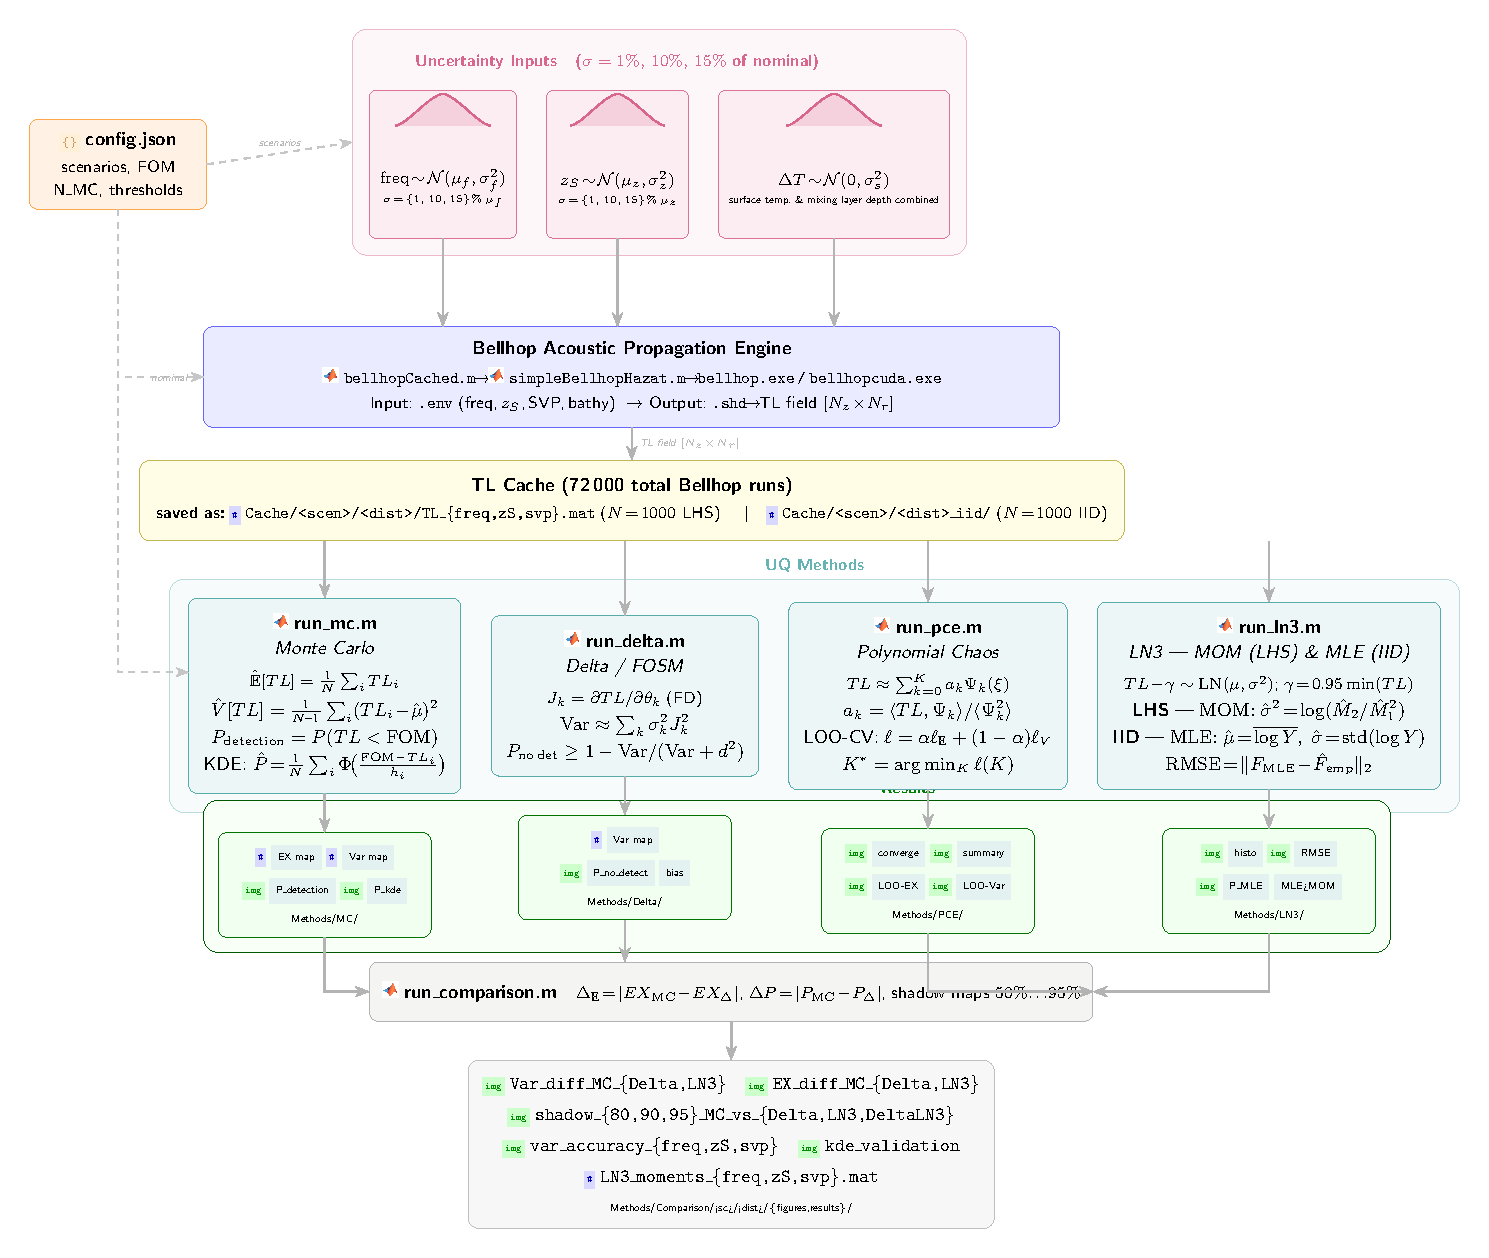
\includegraphics[width=0.82\linewidth]{../docs/block_diagram.pdf}
  \end{center}
\end{frame}

% ── Slide 10: Analytical Validation ──────────────────────────
\begin{frame}{Analytical Validation of Bellhop-FD Jacobian}
  \begin{columns}
    \column{0.52\textwidth}
    
\includegraphics[width=\linewidth]{delta_validation_Normal_5pct.png}
    \captionof{figure}{\footnotesize Bellhop-FD vs.\ analytical waveguide Jacobian,
               Normal\,5\% $z_S$ uncertainty.}

    \column{0.44\textwidth}
    \textbf{Closed-form waveguide:}
    \begin{equation}
      p(r,z) = \frac{i}{H}\sum_m \sin(k_{z,m}z_S)\sin(k_{z,m}z)H_0^{(1)}(k_{r,m}r)
    \end{equation}
    Analytical Jacobian $\partial\TL/\partial z_S$ computed directly.

    \vspace{0.5em}
    \begin{exampleblock}{Result}
      $L_1$ error $< 5\%$ at all uncertainty levels.\\[2pt]
      Bellhop-FD is a valid proxy for the true gradient.
    \end{exampleblock}
  \end{columns}
\end{frame}

% ── Slide 11: Delta Works ────────────────────────────────────
\begin{frame}{Result: Bellhop-FD Delta Succeeds (Flat + Small Perturbation)}
  \begin{columns}
    \column{0.48\textwidth}
    
\includegraphics[width=\linewidth]{baseline/Uniform_1pct/figures/shadow_70_MC_vs_Delta.png}
    \captionof{figure}{\footnotesize Baseline, Uniform\,1\%.
               Left: MC. Right: Bellhop-FD Delta.
               Shadow maps agree closely.}

    \column{0.48\textwidth}
    
\includegraphics[width=\linewidth]{baseline/Uniform_1pct/figures/shadow_70_MC_vs_DeltaLN3.png}
    \captionof{figure}{\footnotesize Baseline, Uniform\,1\%.
               Left: MC. Right: Delta--LN3 hybrid.}
  \end{columns}

  \vspace{0.4em}
  \begin{exampleblock}{Takeaway}
    For \textcolor{successgreen}{\textbf{flat bathymetry + $\leq1\%$ perturbation}},
    Bellhop-FD Delta and Delta--LN3 both match MC ground truth.
    Shadow-probability maps are production-ready.
  \end{exampleblock}
\end{frame}

% ── Slide 12: Delta Fails ────────────────────────────────────
\begin{frame}{Result: Bellhop-FD Delta Fails (Large Perturbation / Slope)}
  \begin{columns}
    \column{0.44\textwidth}
    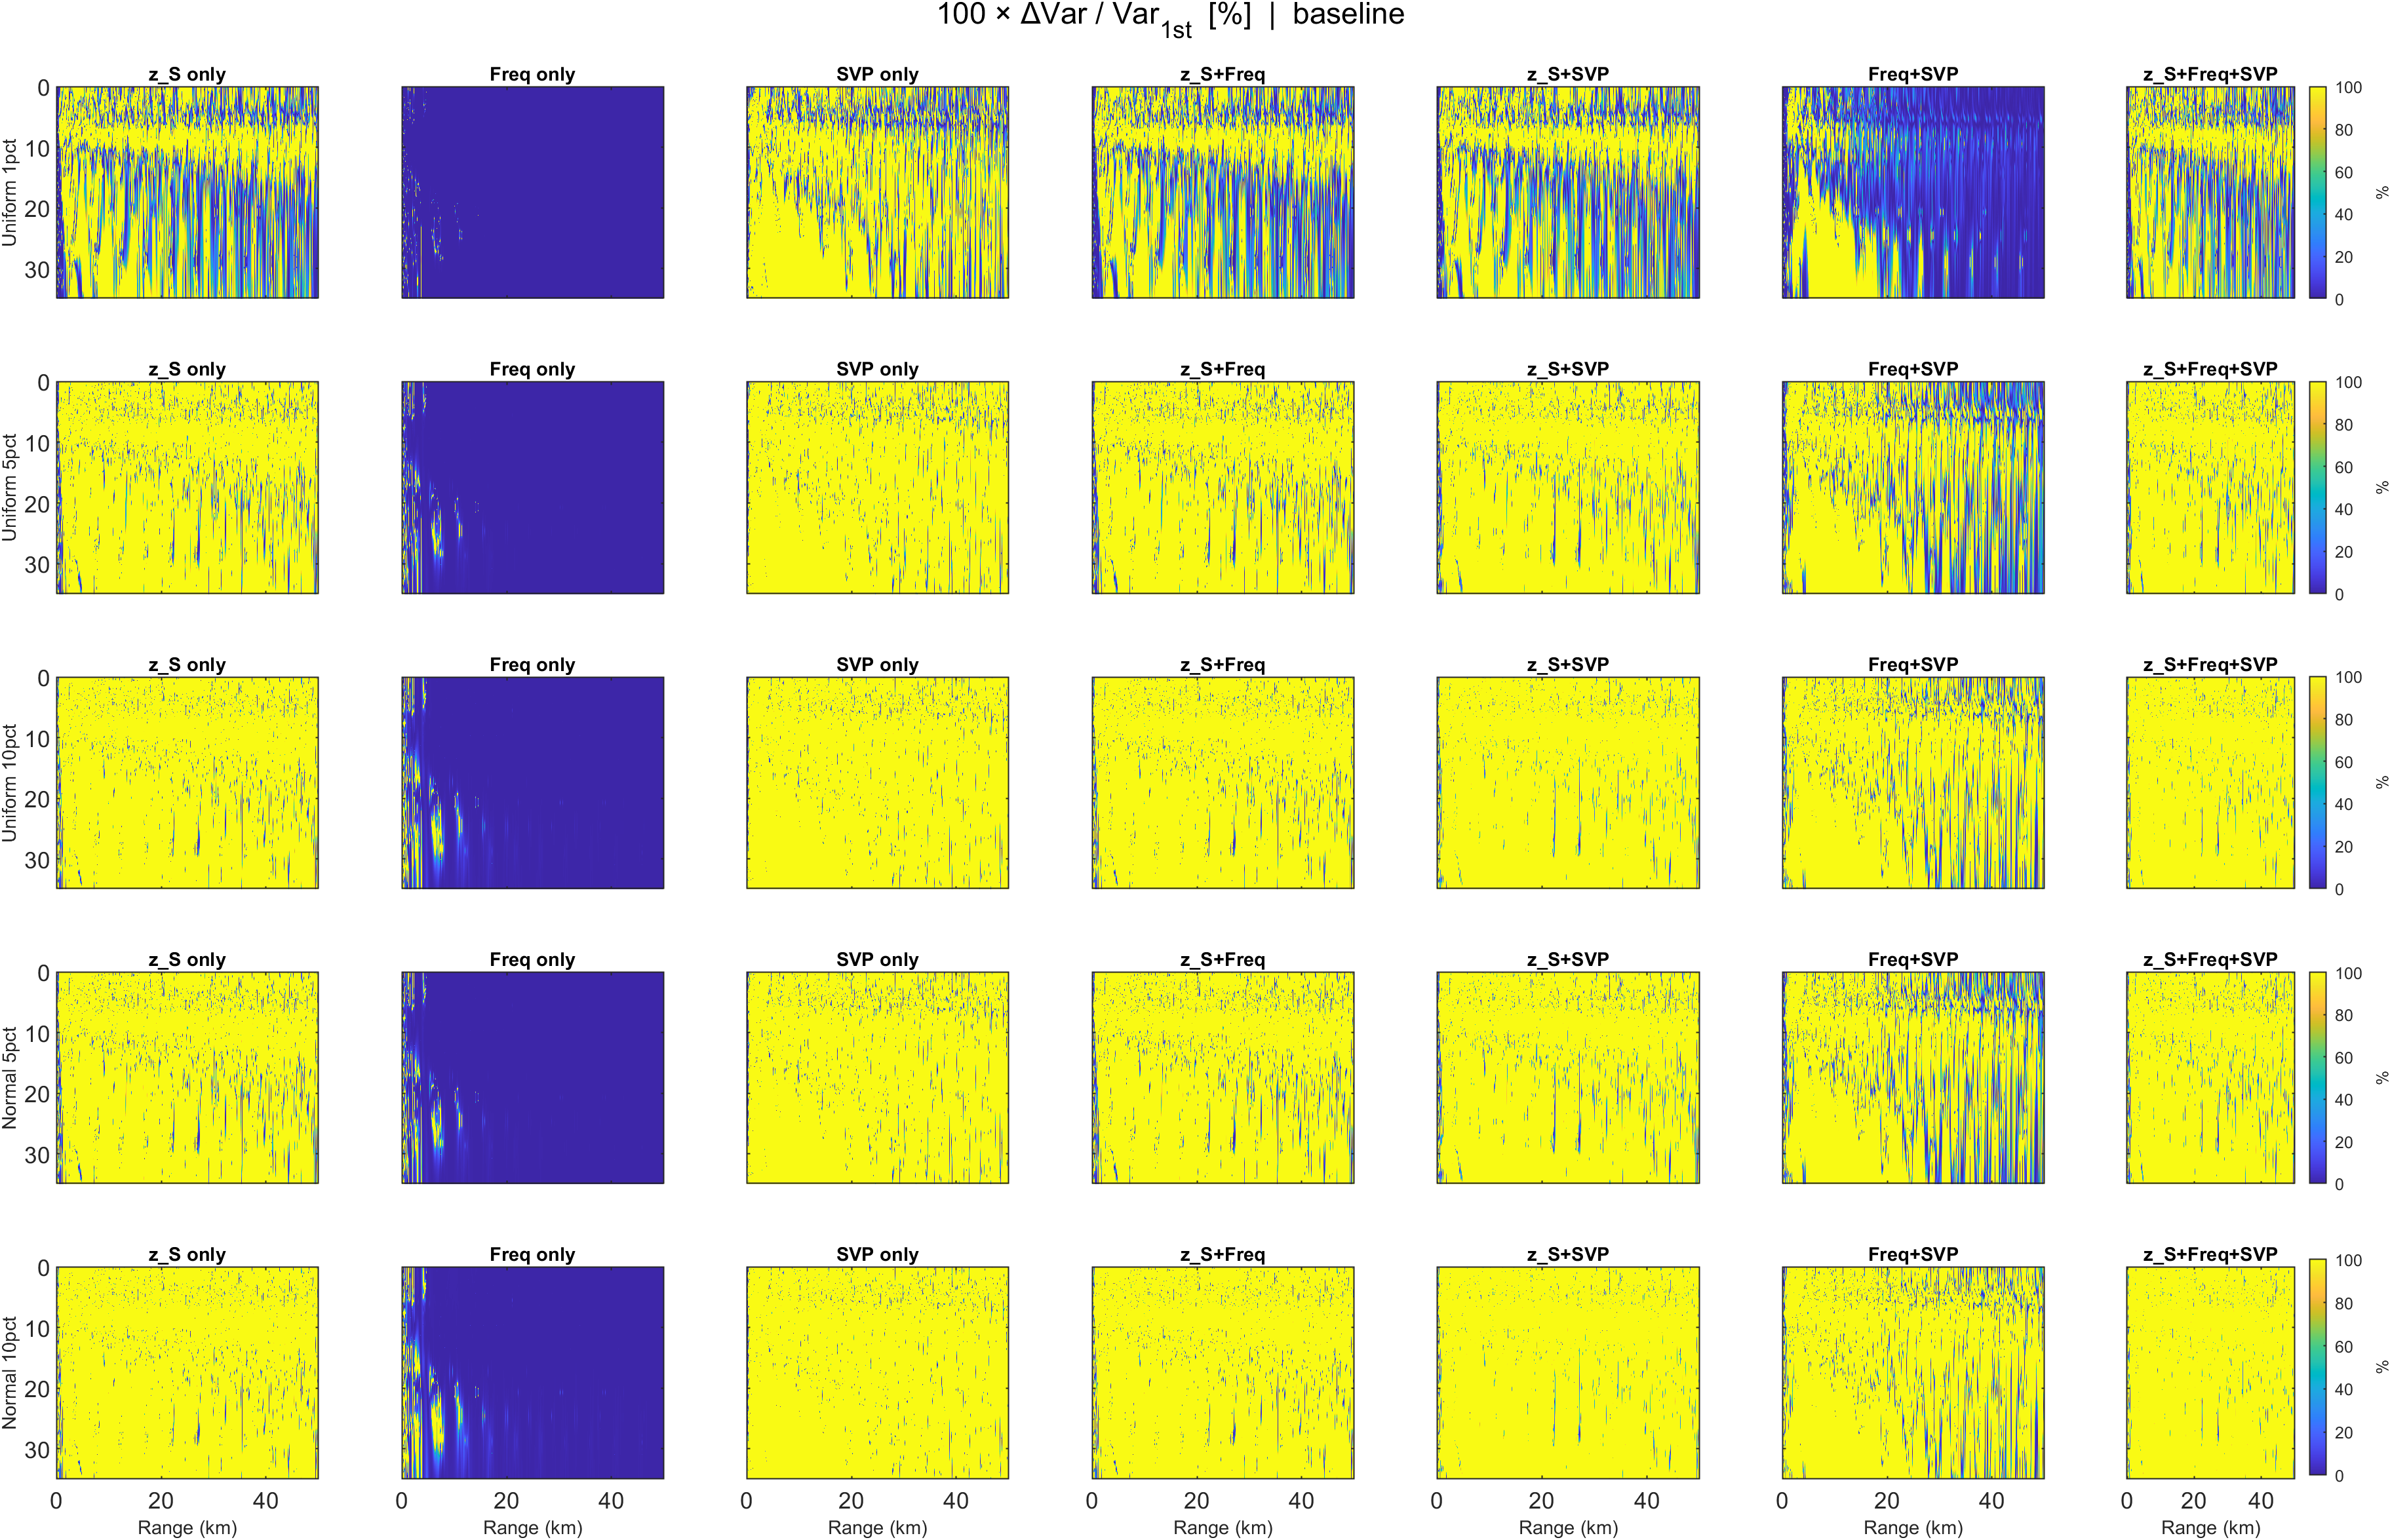
\includegraphics[width=\linewidth]{baseline/delta_order_diff_relative.png}
    \captionof{figure}{\footnotesize Baseline: 2nd/1st order ratio.
               Moderate correction at interference nulls.}

    \vspace{0.3em}
    
\includegraphics[width=\linewidth]{downslope/delta_order_diff_relative.png}
    \captionof{figure}{\footnotesize Downslope: 2nd/1st order ratio.
               Red everywhere --- Taylor series diverged.}

    \column{0.52\textwidth}
    \begin{alertblock}{2nd-order Hessian correction [\%]}
      \begin{tabular}{lcc}\small
        \toprule
        Scenario & 5\% & 10\% \\
        \midrule
        Baseline  & 96.6 & 99.1 \\
        Deep water& 97.0 & 99.2 \\
        Upslope   & 97.5 & 99.4 \\
        Downslope & 96.1 & 99.0 \\
        \bottomrule
      \end{tabular}
    \end{alertblock}
    Values $>$50\%: 1st-order insufficient.\\
    Values $>$96\%: Taylor series has not converged even at 2nd order.

    \vspace{0.4em}
    \textbf{Consequence:} For slope scenarios or $\geq5\%$ perturbation,
    \textcolor{failred}{\textbf{no finite-order Taylor expansion is reliable}}.
  \end{columns}
\end{frame}

% ── Slide 13: PCE Convergence (deep water) ───────────────────
\begin{frame}{Result: PCE Convergence --- Frequency and SVP Converge}
  \begin{center}
    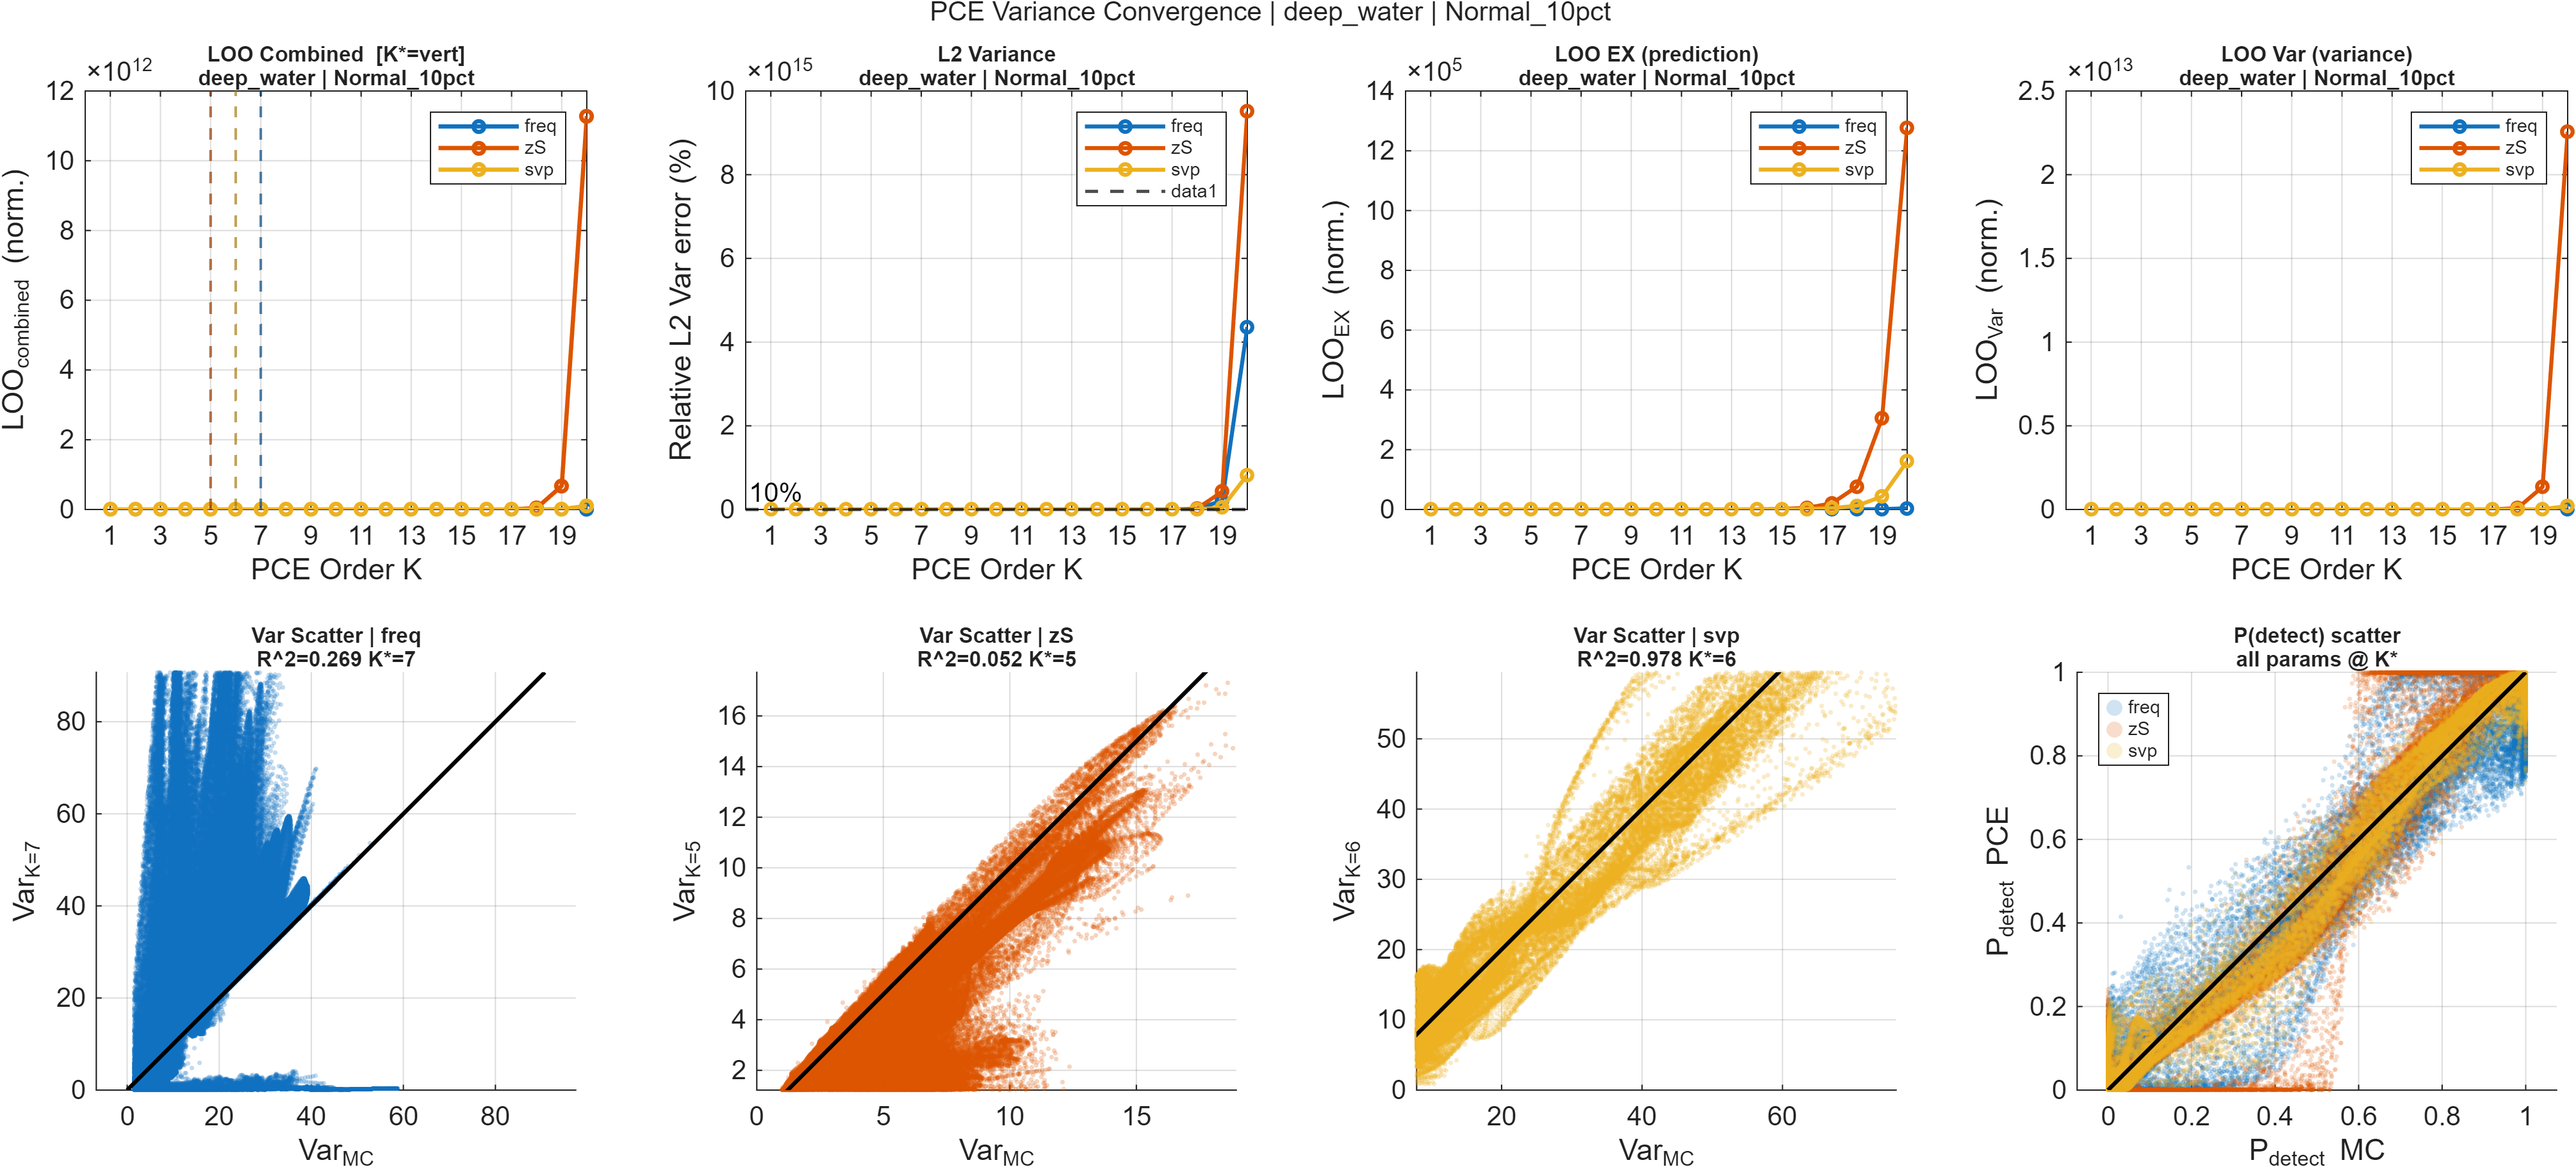
\includegraphics[width=0.82\linewidth]{deep_water/Normal_10pct/figures/pce_convergence_deep_water_Normal_10pct.png}
  \end{center}
  \textbf{Deep water, Normal\,10\%:}
  freq converges at $K^*{=}5$ (blue), SVP at $K^*{=}4$ (green).
  Both reach $L_1 < 10\%$ threshold (dashed line).
  Vertical ticks mark LOO-CV optimal order.
\end{frame}

% ── Slide 14: z_S Anomaly ────────────────────────────────────
\begin{frame}{NEW FINDING: $z_S$ Does Not Converge in Deep Water}
  \begin{columns}
    \column{0.52\textwidth}
    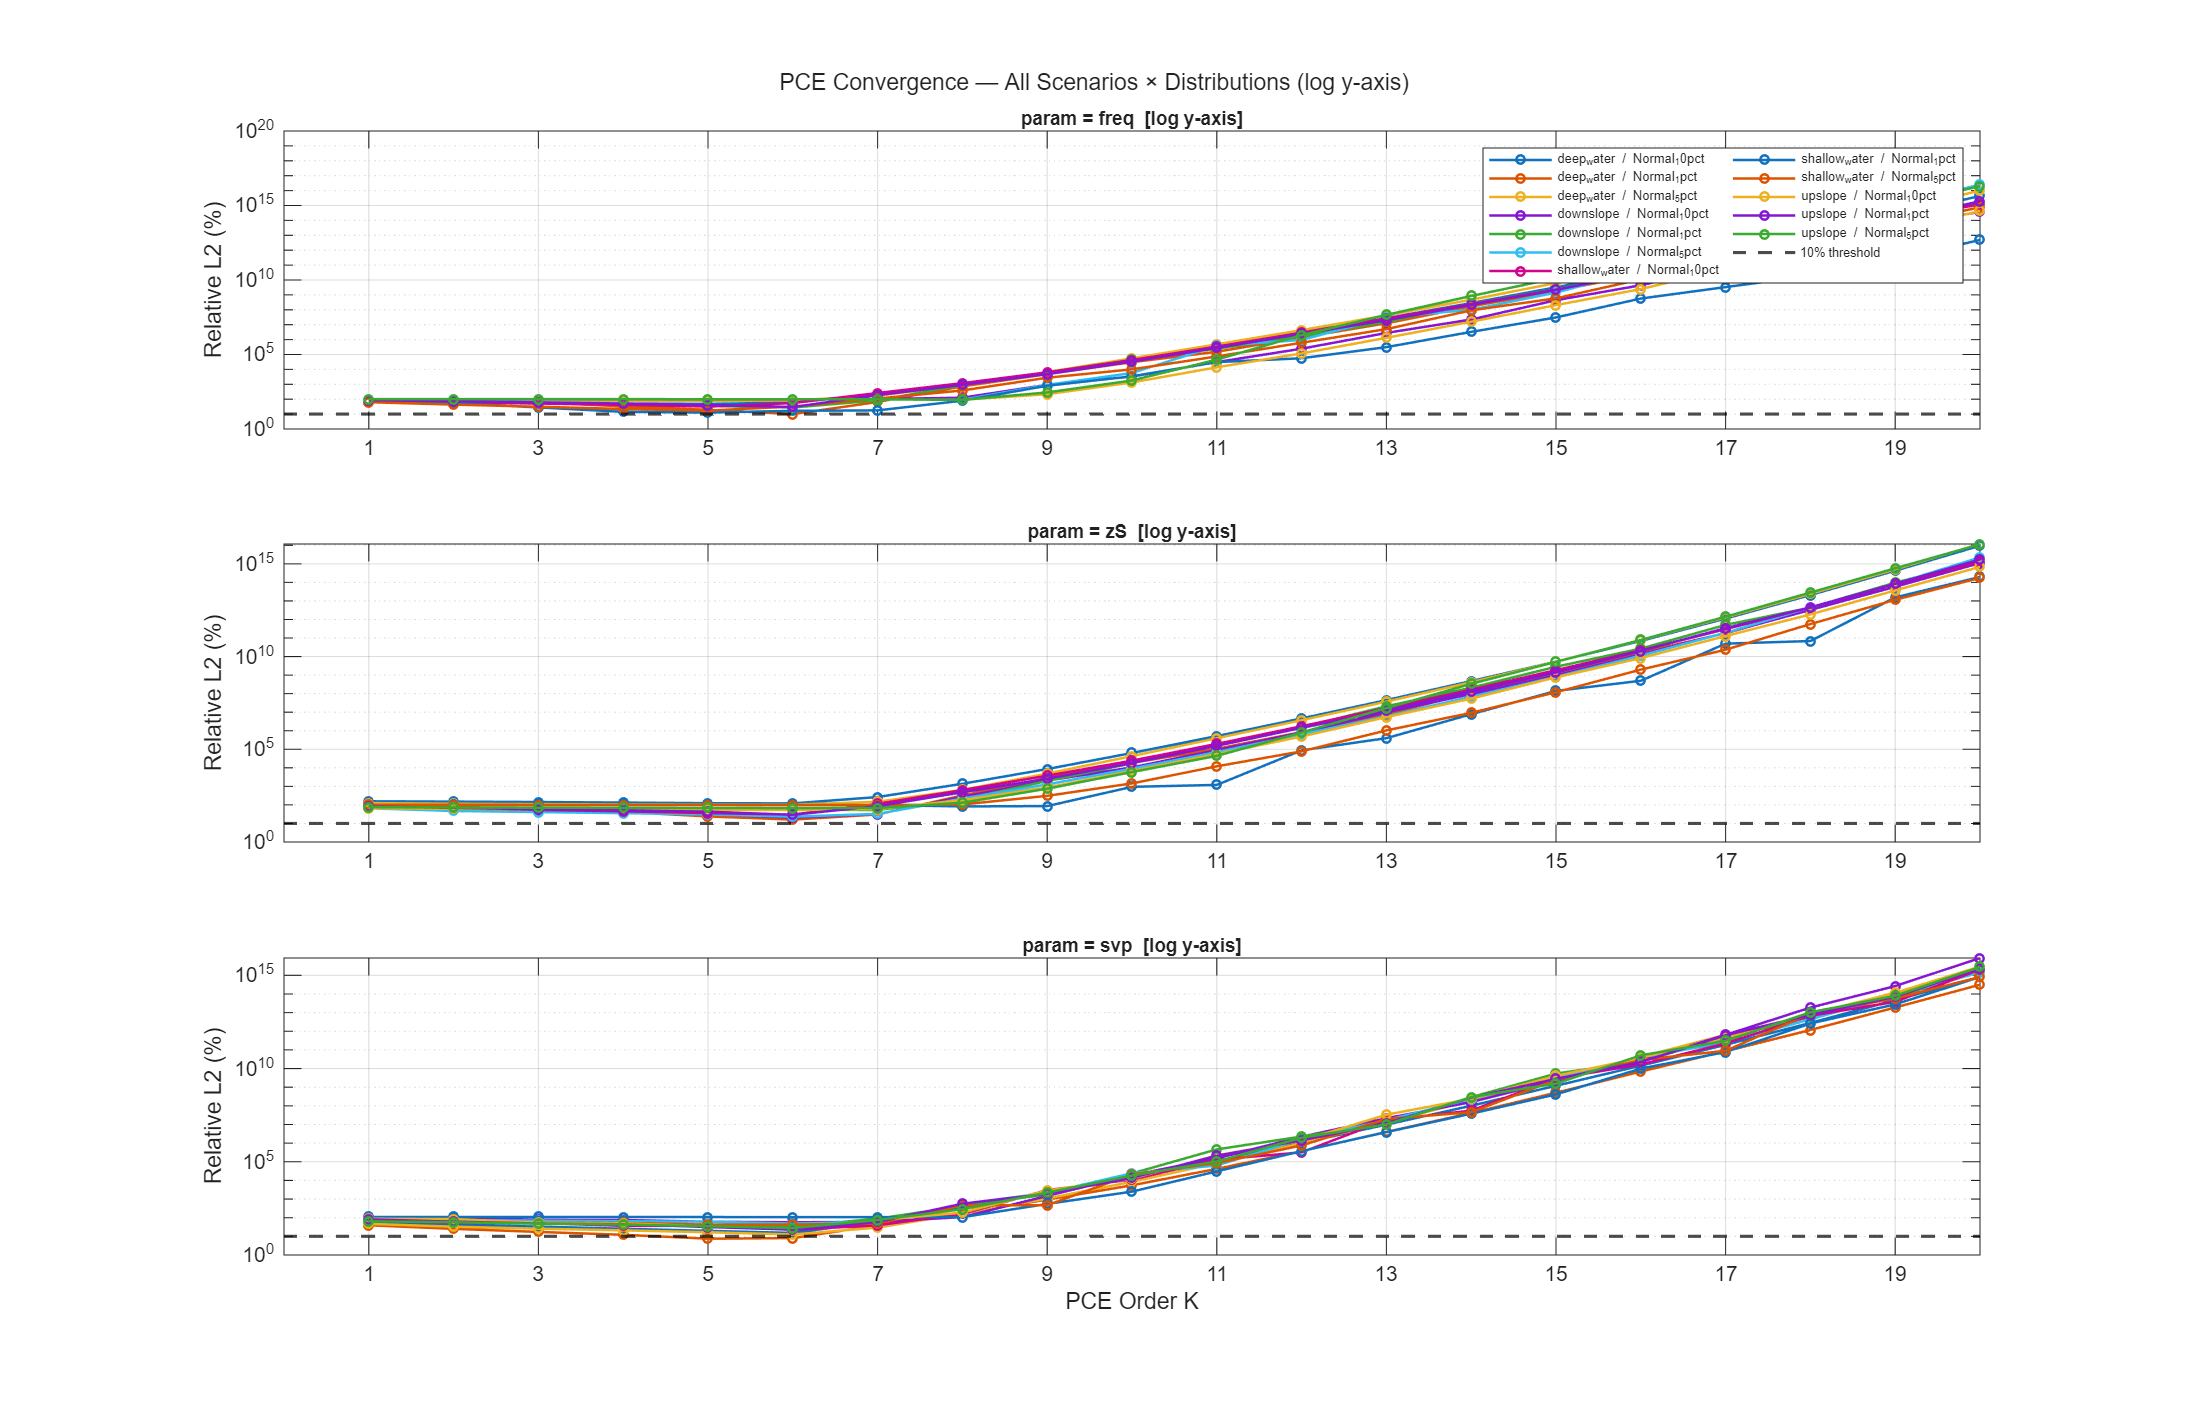
\includegraphics[width=\linewidth]{pce_summary_all.png}
    \captionof{figure}{\footnotesize PCE $L_1$ for all 12 scenario/distribution pairs.
               \textbf{Red curves ($z_S$) never reach the dashed 10\% threshold.}}

    \column{0.44\textwidth}
    \begin{alertblock}{Observation}
      $z_S$ PCE curves remain \emph{above} the $L_1{<}10\%$ threshold at all
      $K \leq 10$ for Normal\,$\geq$5\% in every scenario.
    \end{alertblock}

    \vspace{0.4em}
    \textbf{Physical explanation:}\\
    In deep water, small $z_S$ shifts relative to the SOFAR axis cause
    large nonlinear jumps in modal excitation $\psi_m(z_S)$.
    This creates \emph{non-polynomial} TL response --- no finite-degree
    surrogate can capture it.

    \vspace{0.4em}
    \textbf{Implication:} For $z_S$ uncertainty in deep water,
    \textcolor{failred}{\textbf{full MC is the only reliable method}}.
    Not reported in prior PCE literature.
  \end{columns}
\end{frame}

% ── Slide 15: LN3 Results ────────────────────────────────────
\begin{frame}{Result: LN3 Goodness of Fit}
  \begin{columns}
    \column{0.54\textwidth}
    \begin{block}{KS statistic: $D_\mathrm{KS} = \sup_x |F_\mathrm{emp} - F_\mathrm{LN3}|$}
      \begin{tabular}{lccc}\small
        \toprule
        Scenario & 1\% & 5\% & 10\% \\
        \midrule
        Deep water   & 0.076 & 0.114 & 0.104 \\
        Shallow      & 0.029 & 0.124 & 0.135 \\
        Upslope      & 0.059 & 0.126 & 0.167 \\
        Downslope    & 0.129 & 0.134 & 0.122 \\
        \bottomrule
      \end{tabular}
    \end{block}
    $D_\mathrm{crit} \approx 0.043$ at $N{=}1000$ --- all values exceed this.\\[4pt]
    \textbf{LN3 is formally rejected.}

    \column{0.42\textwidth}
    \begin{exampleblock}{But practically useful}
      $D_\mathrm{KS} \in [0.076, 0.167]$ represents a \textbf{close geometric fit}.

      Rejection is an artefact of large-$N$ sensitivity (the test detects
      deviations irrelevant in engineering practice).
    \end{exampleblock}

    \vspace{0.3em}
    \textbf{Delta--LN3 hybrid:}\\
    Works well for flat scenarios at $\leq5\%$.
    Fails at slope shadow boundaries.
  \end{columns}
\end{frame}

% ── Slide 16: Operational Metrics ────────────────────────────
\begin{frame}{Result: Operational Metrics --- $P_\mathrm{fail}$ Maps}
  \begin{center}
    \begin{subfigure}{0.3\linewidth}
      
\includegraphics[width=\linewidth]{deep_water/Normal_5pct/figures/detect_empirical_freq.png}
      \caption{freq}
    \end{subfigure}
    \begin{subfigure}{0.3\linewidth}
      
\includegraphics[width=\linewidth]{deep_water/Normal_5pct/figures/detect_empirical_zS.png}
      \caption{$z_S$}
    \end{subfigure}
    \begin{subfigure}{0.3\linewidth}
      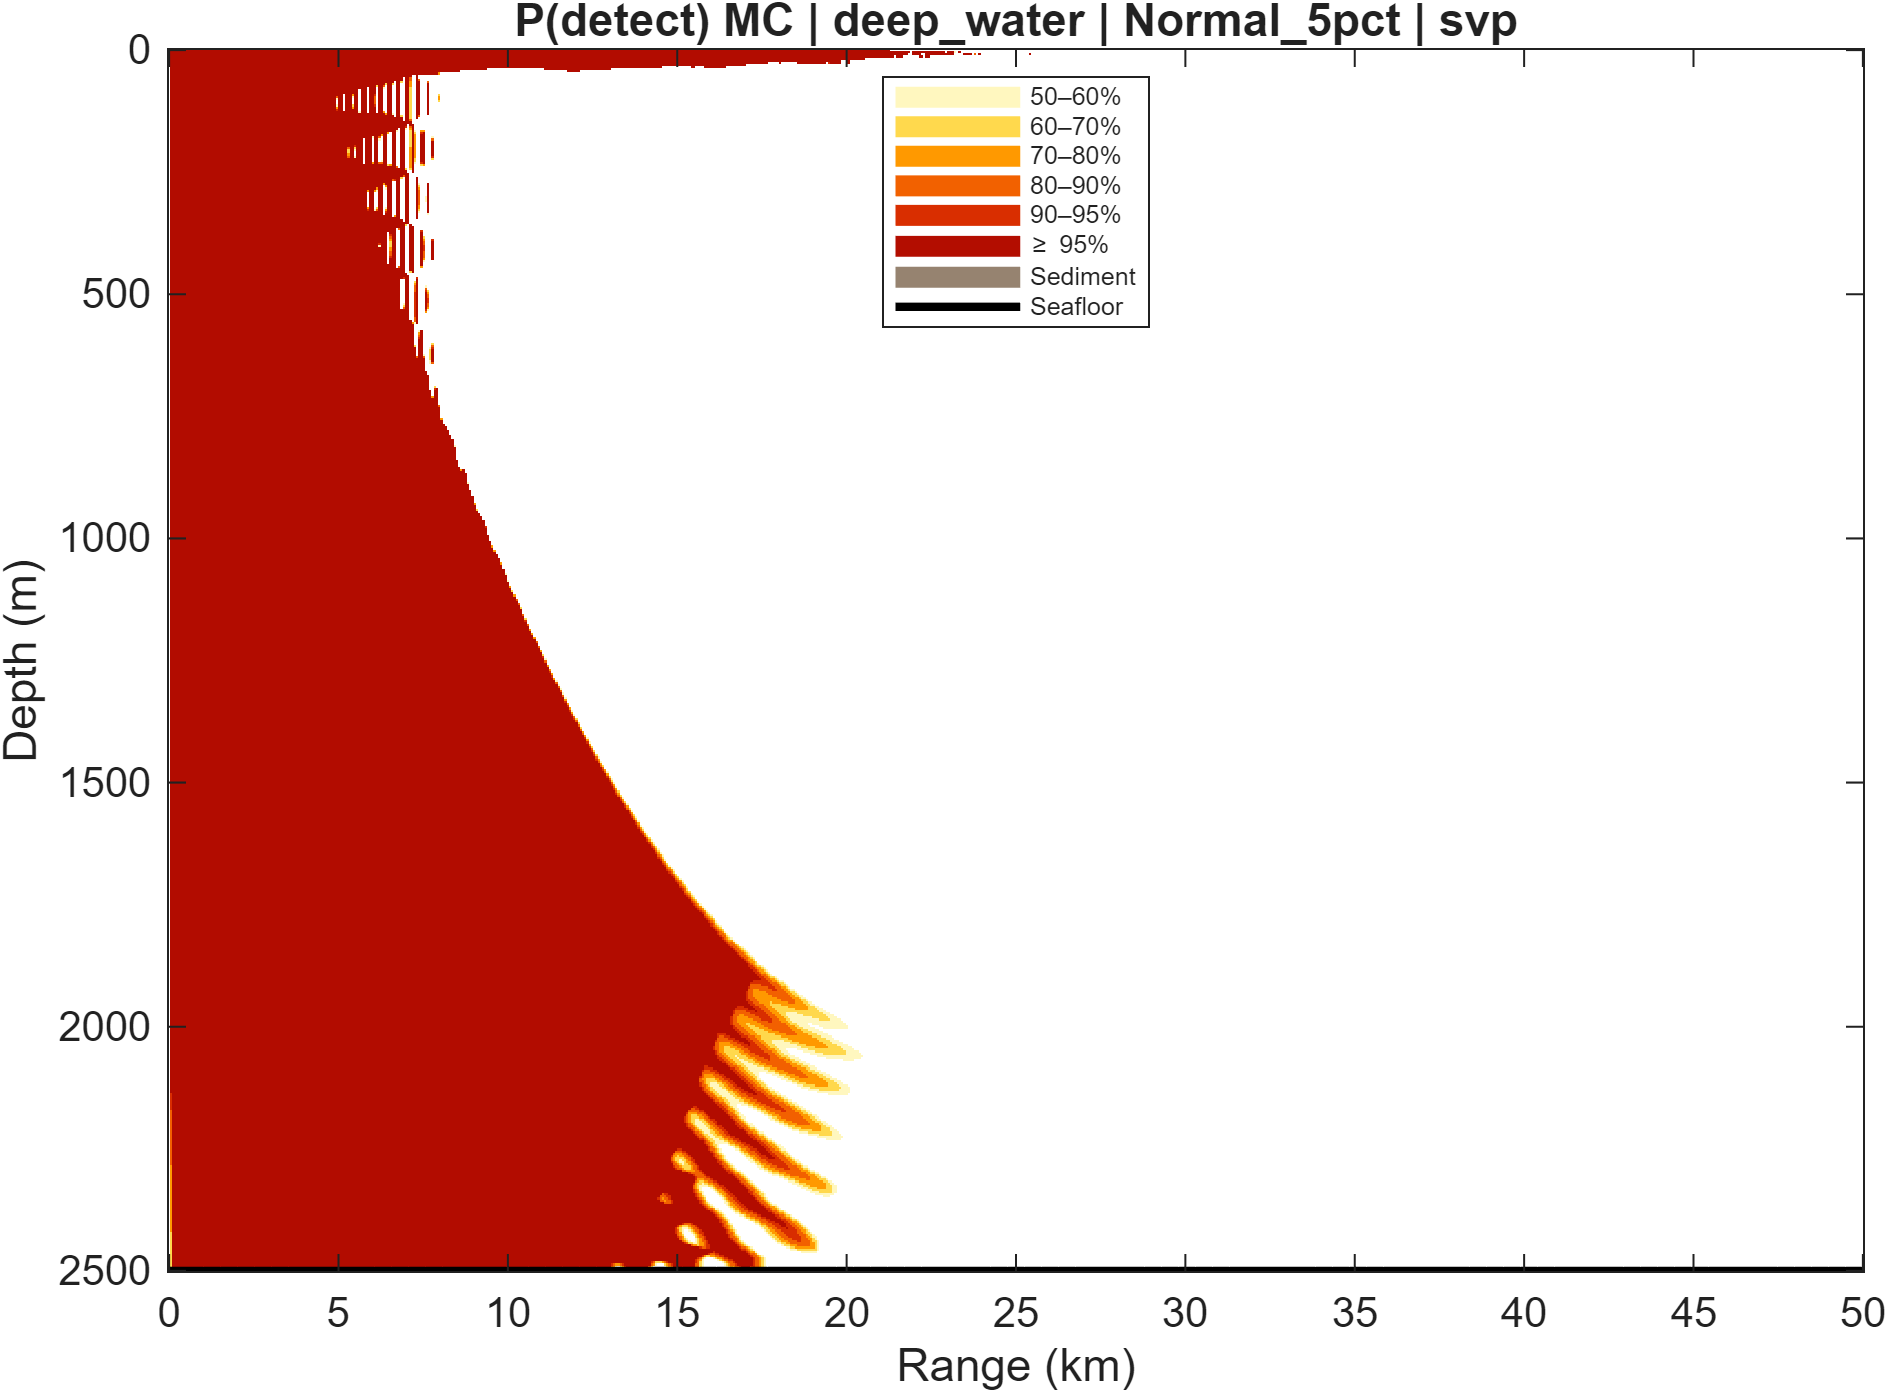
\includegraphics[width=\linewidth]{deep_water/Normal_5pct/figures/detect_empirical_svp.png}
      \caption{SVP}
    \end{subfigure}
  \end{center}
  $P_\mathrm{fail}(r,z) = P(\TL(r,z) > \mathrm{FOM})$, deep water, Normal\,5\%.

  \begin{block}{Key observation}
    $z_S$ (centre) produces the \textbf{largest and most spatially extended} shadow zones
    --- consistent with the PCE non-convergence finding.
    Variance maps alone do not show this: they are symmetric in $\pm\delta$.
  \end{block}
\end{frame}

% ── Slide 17: Recommendation Table ───────────────────────────
\begin{frame}{Method Recommendation by Scenario}
  \begin{center}
  \renewcommand{\arraystretch}{1.35}
  \begin{tabular}{p{2.5cm}ccc}
    \toprule
    \textbf{Scenario} & \textbf{Normal\,1\%} & \textbf{Normal\,5\%} & \textbf{Normal\,10\%} \\
    \midrule
    Flat, freq/SVP pert.
      & \textcolor{successgreen}{\textbf{Delta}}
      & \textcolor{warnyellow}{\textbf{PCE}~$K^*$}
      & \textcolor{warnyellow}{\textbf{PCE}~$K^*$} \\
    Flat, $z_S$ pert.
      & \textcolor{successgreen}{\textbf{Delta}}
      & \textcolor{failred}{\textbf{MC}}
      & \textcolor{failred}{\textbf{MC}} \\
    Slope (up/down)
      & \textcolor{warnyellow}{\textbf{PCE}~$K^*$}
      & \textcolor{failred}{\textbf{MC}}
      & \textcolor{failred}{\textbf{MC}} \\
    \bottomrule
  \end{tabular}
  \end{center}
  \vspace{0.5em}
  \textcolor{successgreen}{$\bullet$}~Bellhop-FD Delta: fast, 6 extra Bellhop runs, flat+small only.\\
  \textcolor{warnyellow}{$\bullet$}~PCE $K^*$: no new runs, surpasses Delta for moderate nonlinearity.\\
  \textcolor{failred}{$\bullet$}~Full MC: gold standard, $N{=}1000$, always reliable.
\end{frame}

% ── Slide 18: Conclusions ────────────────────────────────────
\begin{frame}{Conclusions}
  \begin{enumerate}
    \item \textbf{Bellhop-FD validated}: $L_1 < 5\%$ vs.\ closed-form waveguide.
          Delta method reliable only for flat geometry and $\leq1\%$ perturbation.
    \item \textbf{PCE converges} for frequency and SVP ($K^*{=}3$--6) at zero
          additional Bellhop cost.
    \item \textbf{$z_S$ anomaly (new)}: PCE fails for source-depth uncertainty in
          deep water at all $K \leq 10$ --- attributable to SOFAR modal excitation
          nonlinearity.
    \item \textbf{LN3 practically useful}: $D_\mathrm{KS} < 0.17$ despite formal
          rejection at $N{=}1000$.
    \item \textbf{Report $P_\mathrm{fail}$}, not just variance --- it reveals the
          directional character of acoustic uncertainty.
  \end{enumerate}

  \vspace{0.5em}
  \begin{block}{Future work}
    Design-weighted MLE for LN3 on LHS samples;
    multi-parameter PCE (joint freq+$z_S$+SVP);
    GPU-accelerated Bellhop for $N > 10{,}000$ MC runs.
  \end{block}
\end{frame}

\end{document}
